%!TEX root = ../main.tex
%******************************
%	 Chapter 1 
%*****************************

\chapter{Ageing increases transcriptional noise in CD4$^+$ T cell activation}

\graphicspath{{"../../Dropbox (Cambridge  University)/Figures_for_thesis/Chapter1/"}}

\vfill

\begin{Abstract}
\hspace{-5mm} Ageing is characterised by progressive loss of physiological and cellular functions, but the molecular basis of this decline remains largely unexplored. 
Here, we study how ageing impacts transcriptional dynamics using single-cell RNA-sequencing of over a thousand unstimulated and stimulated naive and effector memory CD4\plus{} T cells from young and old mice. 
Furthermore, we sampled cells from two divergent strains of mice to assess the evolutionary conservation of the molecular ageing signature. 
In young animals, immunological activation drives a transcriptomic switch from variable to tightly regulated gene expression, characterised by a strong up-regulation of a core activation program, coupled to a decrease in cell-to-cell variability. 
The up-regulation of a set of immune response genes is conserved between the two mouse strains as is the decrease in expression variability upon immune activation. 
Ageing significantly perturbed the activation of the core immune response programme by increasing expression heterogeneity across different populations of CD4\plus{} T cells. 
This discovery adds transcriptional noise as an unexplored hallmark of ageing to the list of known phenotypic changes.
\end{Abstract}

\vfill

\newpage

\begin{Comment}
\hspace{-3mm} \textbf{Declaration} This work was a joint effort of the Marioni, Odom, de la Roche and Teichmann labs. 
Celia P. Martinez-Jimenez, Duncan T. Odom, John C. Marioni and Sarah Teichmann designed the study. 
Celia P. Martinez-Jimenez and Aleksandra A. Kolodziejczyk performed preliminary experiments. 
Celia P. Martinez-Jimenez performed all single-cell RNA sequencing experiments displayed in this chapter. 
Hung-Chang Chen and Maike de la Roche provided extensive support during the revision process. 
Hung-Chang Chen performed FACS experiments during the revision process. 
Lovorka Stojic and Frances Connor provided experimental support. Timothy F. Rayner provided technical support. 
Michael J. T. Stubbington performed the T cell receptor and clone analysis. 
Catalina A. Vallejos helped with the statistical analysis by providing additional explanations of the BASiCS model. 
Celia P. Martinez-Jimenez and I interpreted results. 
Celia P. Martinez-Jimenez, Duncan T. Odom, John C. Marioni and I wrote the manuscript. Duncan T. Odom and John C. Marioni supervised the study. 
I performed computational analysis of all data displayed in this chapter and generated all figures with the exception of the FACS analysis (Fig. \ref{fig1:FACS} and Fig. \ref{fig1:EM_Naive_CD4}A-C). 
The paper has been published as:\\

Celia P. Martinez-Jimenez$^\ast$, Nils  Eling$^\ast$, Hung-Chang Chen, Catalina A. Vallejos, Aleksandra Kolodziejczyk, Frances Connor, Lovorka Stojic, Tim F. Rayner, Michael J. T. Stubbington, Sarah A. Teichmann, Maike de la Roche, John C. Marioni, Duncan T. Odom. 
Ageing increases cell-to-cell transcriptional variability upon immune stimulation. \emph{Science}, 1436: 1433-1436, 2017, ($^\ast$ equal contributions)
\end{Comment}

\begin{figure}[hb]
\centering    
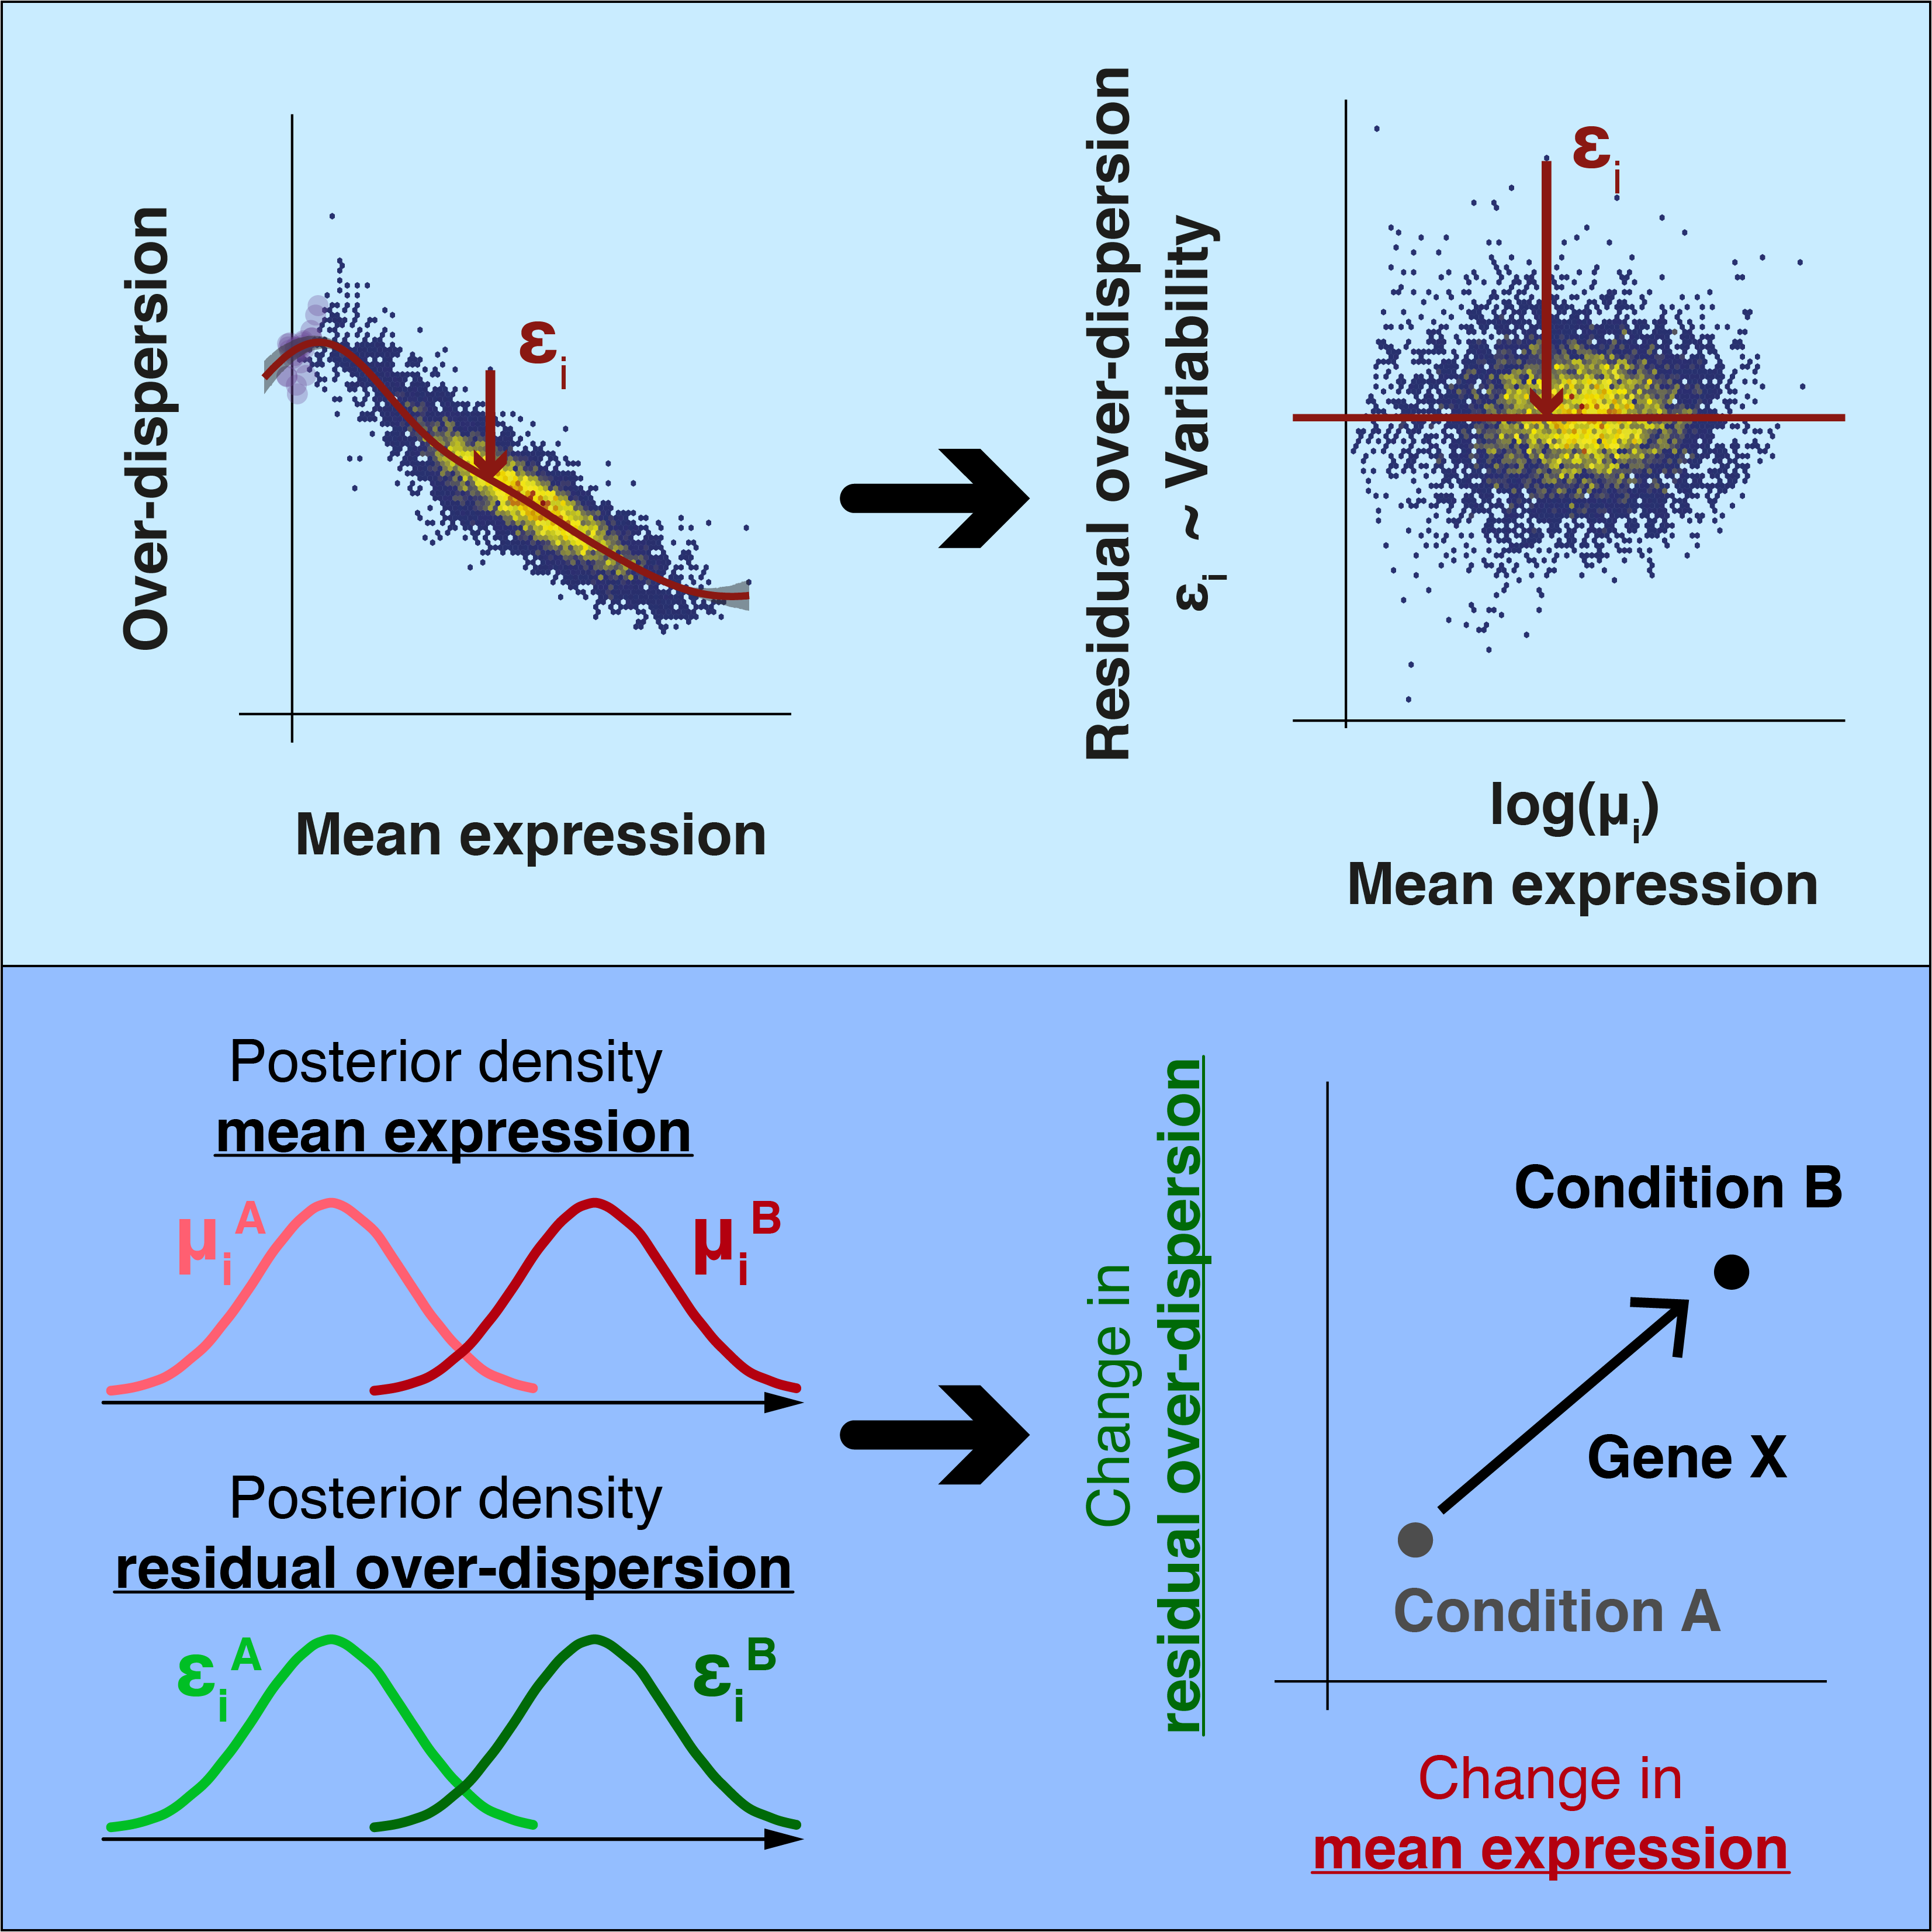
\includegraphics[width=0.8\textwidth]{GraphicalAbstract.png}
\end{figure}

\newpage

% Include different main sections of the first chapter
%!TEX root = ../chapter1.tex
%******************************
%	 Introduction 
%*****************************

\section{Introduction}

Ageing is characterized by the progressive decline of physiological and cellular functions \citep{Lopez-Otin2013, Booth2016}. Nine hallmarks of ageing have been described to determine the ageing phenotype: genomic instability, telomere attrition, epigenetic alterations, loss of proteostasis, de-regulated nutrient sensing, mitochondrial dysfunction, cellular senescence, stem cell exhaustion, and altered intercellular communication \citep{Lopez-Otin2013}. Ageing can have a complex and tissue-specific impact on gene expression levels \citep{Zahn2007}, as seen by microarray expression analyses of collections of mouse CD4$^+$ and CD8$^+$ T cells \citep{Mirza2011}, rat hepatocytes \citep{Tollet-Egnell2000}, mouse and human brain \citep{Lu2004, Lee2000}, human muscle \citep{Welle2003, Zahn2006}, human kidney \citep{Rodwell2004}, human retina \citep{Yoshida2002}, and different species of Drosophila and Caenorhabditis \citep{Mccarroll2004}. For instance, ageing affects distinct functional pathways, even in closely related CD4$^+$ and CD8$^+$ T cells \citep{Mirza2011}. \\

Approaches that analyse the expression of sets of genes on a single-cell basis have more recently suggested that ageing may also alter the cell-to-cell variability of gene expression. Transcriptional noise, RNA processing aberrations, impaired DNA repair, and chromosomal instability can be caused by epigenetic changes occurring in DNA methylation, histone modifications and chromatin remodelling \citep{Lopez-Otin2013}. DNA methylation slightly decreases globally but increases in common disease-related genes over the lifespan of humans \citep{Talens2012}. In mice, around 35\% of assayed genes showed either increased or decreased DNA methylation over ageing displaying strong tissue-specificity of the process \citep{Maegawa2010}. Similarly, ageing introduces changes of histone modifications such as the increase of H4K16ac, H4K20me3 and H3K4me3, as well as the decrease of H3K9me or H3K27me3 \citep{Han2012, Fraga2007}. One well studied system that controls cellular function is the \emph{Sir2} histone deacetlyase which is encoded by seven homologs in mammals \citep{Houtkooper2016}. The chromatin-associated protein SIRT6 in mice has been shown to protect genomic stability by promoting resistance to DNA damage. Loss of this protein induces ageing-realted phenotypes within 4 weeks of murine lifespan \cite{Mostoslavsky2006}.\\

While most studies focused on identifying age-associated gene expression profiles \citep{DeMagalhaes2009}, the role of transcriptional noise during ageing has only been sporadically assessed. Analysis of fifteen genes in terminally differentiated cardiomyocytes suggested that ageing can lead to increased cell-to-cell transcriptional variability \citep{Bahar2006}. In contrast, single-cell analysis of the transcription of six genes in four different hematopoietic stem cell types showed few cell-to-cell changes between old and young animals, leading to the suggestion that transcriptional instability may not be a universal attribute of ageing \citep{Warren2007}. Whether cell-to-cell gene expression variability increases during ageing on a genome-wide basis, particularly for dynamic activation programs, remains largely unexplored.\\

Single-cell RNA sequencing presents a powerful technology to quantify  transcriptional variability in thousands of genes across thousands of cells simultaneously. For example, Kowalczyk \textit{et al.} performed a high-resolution scRNA-seq analysis of hematopoietic stem cells in young and old mice. Here, cell cycle is the primary driver for cell-to-cell variability in gene expression, and ageing decreases the entry of long-term hematopoietic stem cells into G1 phase in a cell-type-specific manner \citep{Kowalczyk2015}.\\ 

To evaluate the impact of ageing on gene expression levels and cell-to-cell transcriptional variability, we selected CD4$^+$ T cells as model system. As explained in \textbf{Box 1}, transcriptional noise is defined as cell-to-cell variability in expression within a homogeneous population of cells. Naive CD4$^+$ T cells are readily isolated as single, phenotypically homogeneous cells when purified from young and aged spleens and can be easily stimulated into a physiologically-relevant activated transcriptional state in vitro. Furthermore, they are maintained in a quiescent state, but have the ability to respond to antigen stimulation with proliferation and effector differentiation, which is essential for life-long maintenance of adaptive immune function against infection and cancer \citep{Swain2012, Kim2014a}. With this, they sit at the root of adaptive immunity and disruption of their transcriptional programme can lead to severe phenotypes during ageing. \\

Previously, comparing gene expression levels in matched tissues from different mammalian species was used as a tool for revealing conserved cell-type-specific regulatory programs \citep{Sudmant2015, Finseth2014, Brawand2011, Flajnik2009}. For instance, a conserved set of response genes has been identified by comparison of bulk gene expression between human and mouse CD4$^+$ T cells after immune activation \citep{Shay2013}. So far, it is not known whether conservation of gene expression levels is also reflected in cell-to-cell variability.\\

Here, we dissect the activation dynamics of naive CD4$^+$ T cells at the single cell level during ageing in two sub-species of mice. With this, we can assay transcriptional dynamics during immune response and how ageing possibly perturbs this system. By comparing our findings across divergent strains of mice, we can assess the evolutionary conservation of the immune response and ageing phenotype. Furthermore, we isolated pure naive and effector memory CD4$^+$ T cells to profile age-related changes in different CD4$^+$ T cell subsets.

\newpage
%!TEX root = ../chapter1.tex
%******************************
%	 Results 
%*****************************

\section{scRNAseq of murine CD4$^+$ T cells}
\subsection*{Single-cell RNA sequencing of CD4$^+$ T cells during activation, ageing and across two mouse species}

To assess the conservation of immune activation programmes, we isolated CD4$^+$ T cells from healthy individuals of two inbred mouse sub-species separated by 1 million years of divergence: the reference C57BL/6J, Mus musculus domesticus (B6); CAST/EiJ, Mus musculus castaneus (CAST)). We characterized their gene expression programmes by single-cell RNA-sequencing (scRNAseq) during ageing in young (~3 months) and old (~21 months) individuals of each strain (Fig. \ref{}). These two sub-species have similar lifespans (23, 24), and CAST mice showed the hallmarks of normal organismal aging observed in B6 mice (25). All mice were healthy at the time of experiments. 

\subsubsection*{Unstimualted CD4$^+$ T cells}

\subsubsection{Naive and effector memory CD4$^+$ T cells}

\subsubsection*{Computational quality control and filtering}

from spleens and characterized their gene expression programs by single-cell RNA-sequencing (scRNA-seq) during aging in young (~3 months) and old (~21 months) individuals of each strain (Fig. 1A, Material and Methods).  

Purified naive CD4+ T cells were either loaded directly into the Fluidigm C1 system, or were loaded three hours after stimulation in vitro with plate-bound anti-CD3$\epsilon$/anti-CD28 antibodies (see Material and Methods). Hereafter, for simplification and clarity, purified unstimulated naive CD4+ T cells will be named naive, and stimulated cells will be named activated. For each species/condition, scRNA-seq experiments were performed using cells isolated from two individual mice. We visually inspected the vast majority of cell-capture sites in each C1 small-integrated fluidic circuit (IFCs, 5-10$\mu$m) using 40x magnification lensing to ensure precise capture of single cells (Fig. S1A and S1B and Material and Methods). We removed low-quality C1 captured cells by evaluating (i) the sequencing depth, (ii) the number of genes detected, (iii) the proportion of sequencing reads mapping to exons and ERCC controls, and (iv) the mitochondrial fraction of reads (Fig. S1C-F). The resulting data showed minimal batch effects (Fig. S1G). Using RNA-sequencing to identify cell-specific marker genes, we removed residual B-cells, CD8+ T cells, and (in activating conditions) non-activated T cells from our analysis (Fig. S1H and S1I, Material and Methods). \\

In contrast to haematopoeitic cells (15), even when activated, virtually all CD4+ T cells are in G1 phase of cell cycle as expected (Fig. S2A). Aged CD4+ T cells showed no clonal expansions (Fig. S2B) or difference in cell size (Fig. S2C) that could impact analysis of gene expression variability (26). Using flow cytometry analysis, we confirmed that 96.4\% of the isolated CD4+ T cells were naive in young B6 (Fig. S2D). Naive CD4+ T cells formed a single, high-purity population in young animals. Old animals had a small population of CD4+ T cells with slightly elevated CD44 levels, reduced CD62L expression, and attenuated activation dynamics (Fig. S2E-G); their removal did not impact our results (Material and Methods) (see below). Upon T cell receptor (TCR) activation in the presence of particular cytokines, naive CD4+ T cells can differentiate into several lineages of functionally different T helper cells (mainly Th1, Th2, Th17, Treg, Tfh) (16, 27). In our data we do not detect any early differentiation in naive and activated CD4+ T cell subsets. In accordance with the literature we found Gata3 but not Th2 cytokines expressed in the majority of cells  (28). Interestingly, the Th1-related genes Tbx21 and Ifng were up-regulated, in an uncoordinated manner, in a small population of activated CD4+ T cells of old animals. This is consistent with a known Th1 bias in CD4+ T cell responses in old mice (29) and humans (30) (Fig. S2H). Furthermore, we did not detect any difference in TCR components/signaling and importantly detected no signs of T cell exhaustion (31), especially in cells isolated from old animals (Fig. S2I). We also ruled out species-specific differences in commitment towards T helper cell lineages (Fig. S2J). \\

After the above analyses and the experimental validation (Material and Methods), a total of 1514 high-quality CD4+ T cell transcriptomes were analyzed across all conditions and species.


\newpage
%!TEX root = ../chapter1.tex
%******************************
%	 Discussion 
%*****************************

\section{Discussion}

How cell-type-specific gene expression programs change during organismal lifespan has long been debated \citep{Bahar2006, Warren2007} but until the beginning of this project, few studies in mammals have quantified the cell-to-cell transcriptome-wide differences that accumulate during ageing \citep{Kowalczyk2015}. Here, we systematically explored the effect of ageing on the dynamic activation program of primary naive CD4\plus{} T cells. We analysed two sub-species of mice, which represents a powerful strategy to identify evolutionarily conserved gene expression programmes \citep{Shay2013}. In contrast to humans, mice were housed in specific pathogen-free facilities that reduces transcriptional changes due to pathogen-induced immune activation \citep{Beura2016}. In this chapter, we therefore profiled the intrinsic effect of ageing on transcriptional regulation in CD4\plus{} T cells.\\

By activating naive CD4\plus{} T cells and quantifying the transcriptional responses of hundreds of single-cells using scRNA-Seq, we confirmed that translation processes and immune response genes are rapidly up-regulated \citep{Asmal2003, Neme2016, Turner2014, Glass2010, Gerondakis2010, Croft2009}. More interestingly, we discovered that transcriptional variability is reduced across thousands of transcripts that otherwise remain stable in mean expression levels. This indicates that immune activation rapidly reduces transcriptional heterogeneity across the population of CD4\plus{} T cells to up-regulate a specific response programme similarly in each individual cell. A similar programme has been identified in iPSC reprogramming where an early phase is characterised by probabilistic events while, later, the transcription of \textit{Sox2} induces a  more deterministic phase \citep{Buganim2012}. Previous studies assayed heterogeneity in immune responses by profiling individual cytokines such as interleukin 2 and interferon \textbeta{} in immune cells. Early responding cells support the activation of surrounding cells by paracrine signalling \citep{Fuhrmann2016, Shalek2014}. In contrast, by profiling thousands of genes, our approach identifies the global collapse of variability as a key event in immune activation.\\

Comparison of gene expression levels across species have been used as a means to identify transcription under strong selection in tissues \citep{Sudmant2015, Brawand2011, Romero2012, Barbosa-Morais2012, Perry2012}, including bulk CD4\plus{} T cells from young mice and humans during immune stimulation \citep{Shay2013}. By profiling two sub-species of mice, we identified a common set of activation genes, including well-characterised immune response genes such as \textit{Il2ra}, that are similarly up-regulated across the two species. Furthermore, using scRNA-Seq allowed us to determine the number of cells that express a certain gene. With this, we newly revealed that immune stimulation results in the vast majority of cells within each species up-regulating the set of evolutionarily conserved genes. In contrast, we discovered that genes whose mean expression was up-regulated in a species-specific manner were often activated in only a small fraction of cells, suggesting weaker selection. Indeed, species-specific up-regulated genes showed no functional enrichment. This discovery suggests a novel defining feature of functional target genes: coherent transcriptional up-regulation across a population of cells. \\

Many attempts have been made to identify transcriptional signatures associated with ageing \citep{DeMagalhaes2009, Magalhaes2009, Chen2013, Kowalczyk2015}. On a genome-wide basis, we observed that ageing has minimal effects on mean expression levels in unstimulated and stimulated CD4\plus{} T cells. However, in the core set of activated genes, in both species and in distinct CD\plus{} T cell subsets, we found a markedly more heterogeneous transcriptional response to stimulation in older mice. This increased heterogeneity was driven by ageing associated differences in the (reduced) fraction of cells across the population that express these response genes. Instead of detecting structured heterogeneity, characterised by some cells not responding to the stimulus, we observed that all cells from old animals responded, but in contrast to young cells, failed to homogeneously up-regulate the response programme. \\

High numbers of CD4\plus{} T cells are needed to combat infection and cancer. The discovery that CD4\plus{} T cells from aged mice are unable to up-regulate a core activation program robustly may in part explain the decrease of immune function observed in aged mammals \citep{Goronzy2013, Nikolich-Zugich2018}. More generally, in the context of the current understanding of transcriptional dysregulation and chromatin destabilization during ageing \citep{Booth2016}, increased cell-to-cell transcriptional variability is a major, and largely unexplored, intrinsic factor.\\

Following the publication of this study, several mechanisms for the increase in transcriptional variability during ageing have been proposed. In one study, the increase in transcriptional variability during ageing was confirmed in human pancreatic \textbeta{}-cells. A possible mechanism for this increase in variability is so called "fate drift" of \textbeta{}-cells to resemble \textalpha{}-cells. During ageing, \textbeta{}-cells that are defined by their expression of the hormone \emph{insulin} increase expression of the hormone \emph{glucagon}, the characteristic hormone of \textalpha{}-cells. This atypical hormone expression can result in increased transcriptional noise during ageing in the pancreas \citep{Enge2017}. Another study by Desch\^{e}nes and Chabot, 2017 proposed that the stochastic shortening of telomeres during ageing introduces variation in a process termed Telomere Position-Effect On Long Distance (TPE-OLD). 	TPE-OLD regulates the expression of genes 10 Mb into the chromosome and its variation can lead increased transcriptional heterogeneity during ageing \cite{Deschenes2017}. Further, Cheung \emph{et al.}, 2018 profiled a variety of epigenetic marks in different subsets peripheral blood mononuclear cells (PBMCs) in young (< 25 years) and old (> 65 years) humans at single-cell resolution \citep{Cheung2018}. Analysis of 40 chromatin marks in 20 cell types revealed a separation between young and old individuals and an enrichment in most chromatin marks during ageing. Furthermore, they found an increase in cell-to-cell variability for the majority of chromatin marks in aged individuals. The authors proposed a possible role for polycomb-repressive complexes (PRC) in increasing epigenetic variation and showed that PRC-mediated H3K27me3 deposition explains the increase in transcriptional variability that we reported in this chapter \citep{Cheung2018}.\\

While an increase in transcriptional noise has been shown to be associated with tissue ageing in pancreas and the immune system, a more complete view of whole-organism tissue ageing is missing. One study that begins to address this profiled changes in transcriptional noise in multiple cell types in young and old mice \citep{Angelidis2018}. Not only did they confirm the increase in transcriptional noise during ageing in CD4\plus{} T cells but also observed this shift in a variety of cells types associated to the lung (e.g. NK cells, macrophages, dendritic cells, endothelial cells, smooth muscle cells and neutrophils) \citep{Angelidis2018}. This analysis validates increased transcriptional noise as a major hallmark of ageing. \\

The major drawback in this chapter was the inability to profile all immune response genes for changes in variability due to the dependency of the over-dispersion parameter on the mean expression parameters (see \textbf{Section \ref{sec0:BASiCS}}). The simple approach to only profile genes with stable mean expression levels during immune activation excluded all immune-associated genes from analysis. These are generally the genes that define T cell phenotypes and functionality. In the next chapter, I will therefore describe an extension of the BASiCS framework to include genes that display changes in mean expression by regressing out this mean-variability dependency.






